\newpage
\section{HIMA OPC Server}

Setting up the server

\begin{figure}[!htb]
    \centering
    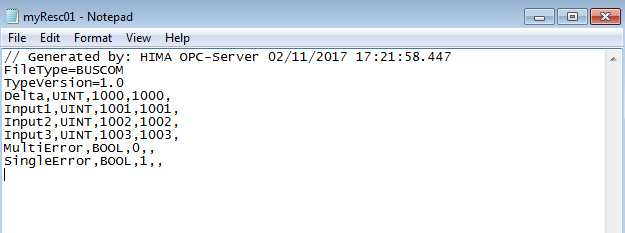
\includegraphics[scale=0.9]{images/del3}
     \caption{Output from OPC-Server}
\end{figure}

\subsection{Determining the IP address of F8625}
Determining the IP address of the communcation module is determined by the last two digits of the resource. The resource name must have eight characters and the last two characters must be numbers, the last two number characters decide two IP address. The calculation is shown in page 6 of the F88625 manual.
\textbf{For module 1:}
Host address = (the last two digits of the resource) * 2 +1 

\textbf{For Module 2:}
Host address = (the last two digits of the resource) *2 +2


\subsection{Controlling the diodes from the OPC-client}
Figure \ref{Eq:2}  shows both diodes on when the difference between 2 or more inputs is larger than the set value (Delta), Multiple Error.
\begin{figure}[!htb]
    \centering
    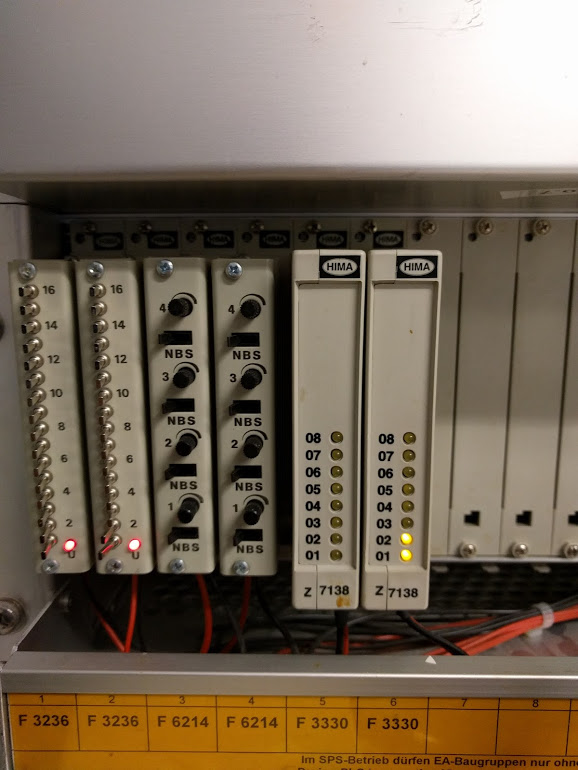
\includegraphics[scale=0.4]{images/ME}
     \caption{MultiError}
     \label{Eq:2}
\end{figure}

\subsection{Why OPC server?}
The HIMA OPC server acts as a transmission interface between 
systems and manufactures without either of them having to know each other's native protocol.

